The code is provided in the separate file \textbf{source.py}.

\begin{figure}[H]
    \centering
    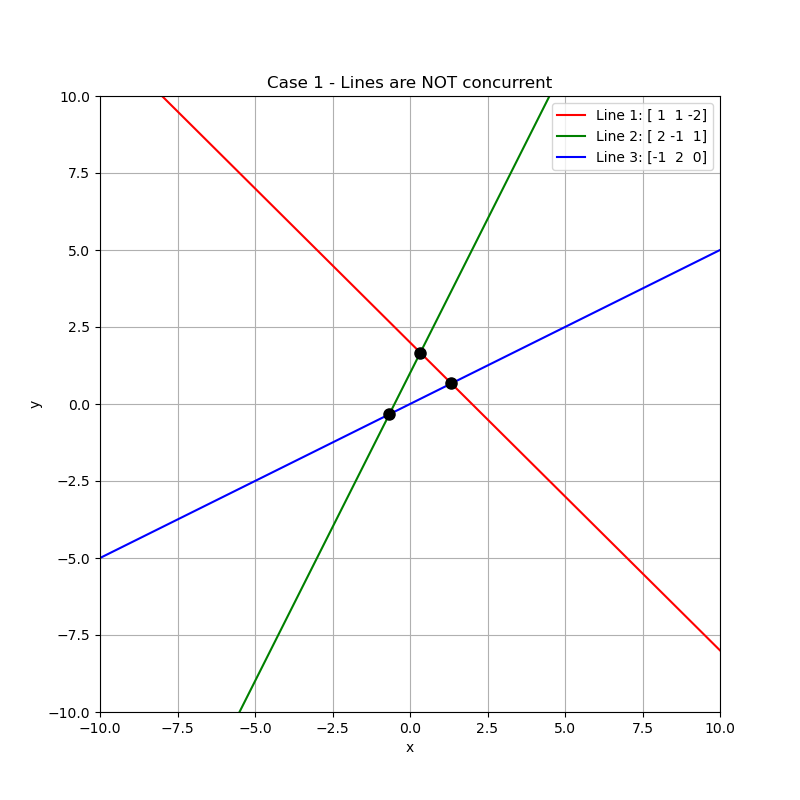
\includegraphics[width=0.4\textwidth]{../Assets/Case_1.png}
    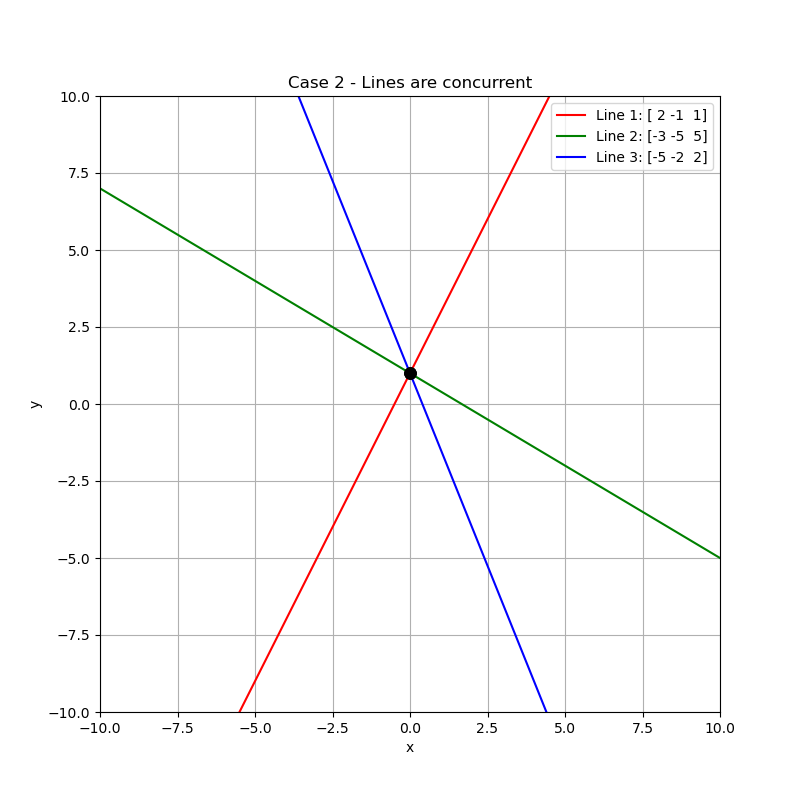
\includegraphics[width=0.4\textwidth]{../Assets/Case_2.png}
    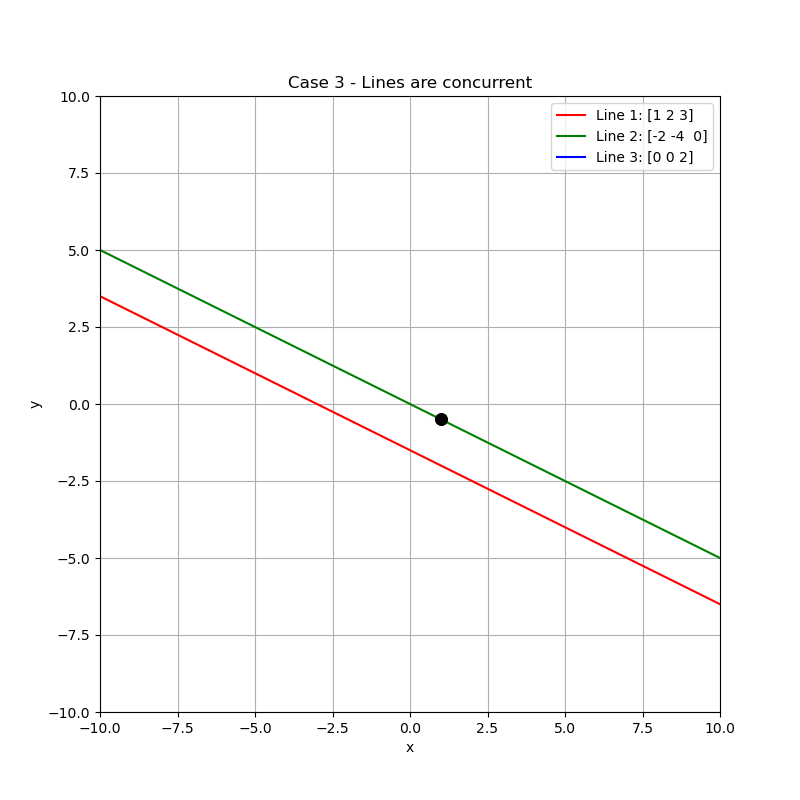
\includegraphics[width=0.4\textwidth]{../Assets/Case_3.png}
    \caption{Intersection of lines \( l \) and \( m \)}
    \label{fig:intersection}
\end{figure}

In the third case lines 2 and 3 are parallel, so the intersection point is not defined.